\chapter{Methodology}

In order to achieve the objectives presented in Section \ref{sec:Objectives}, this chapter establishes the methodological framework followed throughout this thesis. The purpose of this chapter is to define how the separation problem is approached, which data are used and how the different experiments are designed and evaluated.

To ensure that the study is carried out in a realistic and reproducible way, the chapter first describes the general approach adopted for the problem, including the separation algorithms considered and their motivation. Then, the two main datasets used in the project are discussed.  Finally, the chapter describes the experimental procedure followed in each test, including signal selection process, signal conditioning, mixing and evaluation metrics. For reference, Figure \ref{fig:experimental_pipeline} shows a block diagram of procedure followed throughout the thesis for the experiments.
\\
\begin{figure}[H]
    \centering
    \makebox[\textwidth][c]{%
    \resizebox{1.20\textwidth}{!}{%
    \begin{tikzpicture}[
        block/.style={
            draw,
            rectangle,
            minimum width=3.0cm,
            minimum height=2cm,
            text width=2.7cm,
            align=center,
            font=\small
        },
        arrow/.style={-{Stealth}, thick},
        label/.style={font=\small, above}
    ]

    \node[block] (sig) {Signal selection\\and \\ conditioning};
    \node[block, right=1.2cm of sig] (mix) {Mixture model};
    \node[block, right=1.2cm of mix] (pre) {Preprocessing};
    \node[block, right=1.2cm of pre] (sep) {Separation\\algorithm};
    \node[block, right=1.2cm of sep] (ass) {Assessment};

    \draw[arrow] (sig.east) -- node[label]{$s_1, s_2$} (mix.west);
    \draw[arrow] (mix.east) -- node[label]{$c_1, c_2$} (pre.west);
    \draw[arrow] (pre.east) -- node[label]{$z_1, z_2$} (sep.west);
    \draw[arrow] (sep.east) -- node[label]{$\hat{s}_1, \hat{s}_2$} (ass.west);

    \end{tikzpicture}
    }%
    }
    \caption{Block diagram of pipeline followed for the experiments in this thesis.}
    \label{fig:experimental_pipeline}
\end{figure}

\section{Problem modeling}
\label{ch:problem_modeling}
This section introduces the signal model used throughout the thesis. Rather than attempting to describe the full physiological complexity of reinnervated EMG, the aim is to define a simplified mathematical framework that captures the main aspects relevant to source separation. The modeling approach is developed progressively. first, a general linear mixture model with multiple sources and observations is presented. After that, it is reduced to the two-source, two-channel case. Finally, it is specialized to the scenario of interest for the study, in which the target source is weaker and the donor-muscle contribution dominates one of the observed channels. For clarity, in the 2D cases, $\mathbf{s_1}$ denotes the \textbf{target flap-related source} and $\mathbf{s_2}$ the \textbf{donor-muscle source}. 
\clearpage

\subsection{General model}
The recorded EMG channels are modeled as mixtures of latent source signals. In a general setting, let $s_1(t), s_2(t),...,s_n(t)$ denote the underlying physiological sources and let $x_1(t),x_2(t),...,x_n(t)$ denote the observed channels. Each observation is expected to contain a weighted contribution of all sources, together with an additive noise term. This model can be expressed as a system of linear equations as shown in equation \ref{eq:inst_general_system}. Under the simplest instantaneous linear model, the observation vector can also be written as a linear transformation of the source vector plus noise, as shown in equation \ref{eq:inst_general_model}.
\begin{equation}
\left\{
\begin{aligned}
x_1(t) &= a_{11}s_1(t) + a_{12}s_2(t) + \cdots + a_{1n}s_n(t) + n_1(t) \\
x_2(t) &= a_{21}s_1(t) + a_{22}s_2(t) + \cdots + a_{2n}s_n(t) + n_2(t) \\
&\ \,\vdots \\
x_n(t) &= a_{n1}s_1(t) + a_{n2}s_2(t) + \cdots + a_{nn}s_n(t) + n_n(t)
\end{aligned}
\right.
\label{eq:inst_general_system}
\end{equation}
\begin{equation}
    x(t)=As(t)+n(t)
    \label{eq:inst_general_model}
\end{equation}

\noindent where $a_{ij}$ represents the contribution of source $j$ to observation $i$ and $A$ denotes the mixing matrix formed by the $a_{ij}$ coefficients.

This representation alone is not intended to fully describe the physical propagation of EMG through human tissue. Since the electrical activity generated by nearby muscles does not reach all electrodes under exactly the same conditions, each observation may contain contributions that are not only attenuated, but also slightly delayed with respect to one another. These delays may arise from differences in propagation path, electrode position, tissue properties and the spatial distribution of the underlying sources \cite{muceli_tutorial_2024}. As a result, the contribution of a given source to one channel does not necessarily appear at the same instant in another channel.

To account for this effect, the instantaneous mixture model can be extended by introducing delayed source terms. This leads to a convolutive mixture model, in which each observation depends on present and past values of the sources. However, for the purposes of this thesis, it is enough to only consider a single delay per channel and observation. This delay is implemented in equations \ref{eq:conv_general_system} and \ref{eq:conv_general_model}, which represent the extended convolutive version of \ref{eq:inst_general_system} and \ref{eq:inst_general_model}.

\begin{equation}
\left\{
\begin{aligned}
x_1(t) &= a_{11}s_1(t) + a_{12}s_2(t-\tau_{12}) + \cdots + a_{1n}s_n(t-\tau_{1n}) + n_1(t) \\
x_2(t) &= a_{21}s_1(t-\tau_{21}) + a_{22}s_2(t) + \cdots + a_{2n}s_n(t-\tau_{2n}) + n_2(t) \\
&\ \,\vdots \\
x_n(t) &= a_{n1}s_1(t-\tau_{n1}) + a_{n2}s_2(t-\tau_{n2}) + \cdots + a_{nn}s_n(t) + n_n(t)
\end{aligned}
\right.
\label{eq:conv_general_system}
\end{equation}

\begin{equation}
    x(t)=A_{\tau}s(t)+n(t)    
    \label{eq:conv_general_model}
\end{equation}

\noindent where $\tau_{ij}$ denotes the delay associated with  the contribution of source $j$ to travel to observation $i$. The notation  $A_{\tau}$ is used as a compact representation of the delayed mixing model.

While the previous equations describe the general $n$-source case, the remainder of this chapter focuses on a two-source, two-observation model. This reduced formulation is the simplest one in which source separation remains meaningful and it already captures the main features of the problem studied in this thesis. Equation \ref{eq:2d_conv_general_system} shows the general delayed model in the two-dimensional case.
\begin{equation}
\left\{
\begin{aligned}
x_1(t) &= a_{11}s_1(t) + a_{12}s_2(t-\tau_{12}) + n_1(t) \\
x_2(t) &= a_{21}s_1(t-\tau_{21}) + a_{22}s_2(t) + n_2(t) 
\end{aligned}
\right.
\label{eq:2d_conv_general_system}
\end{equation}

\subsection{Symmetric attenuation}
\label{sec:symmetric_attenuation}

The model introduced in the previous section can be considered as a standard \textit{Blind Source Separation (BSS)} setting, since no prior information is assumed about the values of the mixing coefficients $a_{ij}$ or about the properties of the original sources. However, given that this thesis aims to study specific scenarios related to the problem of interest, the current model proposed can be further improved by including additional information. 

In invasive EMG (or in surface EMG of relatively isolated muscles), each recorded channel can be approximated as the sum of the intended target source and an interfering contribution from the other source. Although invasive recordings are usually more selective than surface EMG, they do not guarantee perfect source isolation, since the adjunct muscular activity can still interfere with the measured channel 
\cite{m_consensus_nodate,l_analysis_2020}. Each channel is assumed to be dominated by its corresponding source, so the direct coefficients are simplified to $a_{ii}=1$. If both muscles are equally dominant an their interference is balanced, the off-diagonal terms can be expressed by a parameter $\beta$, where $a_{ij}=\beta$ for $\forall i\neq j$. Equation \ref{eq:2d_conv_beta_system} expresses the new model after taking into account these two considerations.

\begin{equation}
\left\{
\begin{aligned}
x_1(t) &= s_1(t) + \beta s_2(t-\tau_{12}) + n_1(t) \\
x_2(t) &= \beta s_1(t-\tau_{21}) + s_2(t) + n_2(t) 
\end{aligned}
\right.
\label{eq:2d_conv_beta_system}
\end{equation}

\subsection{Weak-source regime}
\label{sec:weak_source_regime}

Unfortunately, in reinnvervated muscle configurations, the interaction between the two muscular contributions is not necessarily balanced. In some cases, one source may display a stronger influence on the observed mixtures that the other, sot he coupling between channels cannot always be assumed to be symmetric. In fact, in procedures like VDMT, the contribution of the auxiliary muscle over the target flap-related source ($a_{12}$) is generally greater than the reverse interaction ($a_{21}$), which can barely be noticed in the auxiliary muscle observation. Mathematically, this can be expressed as $\mathbf{a_{21}=\alpha}$ with $\mathbf{\alpha<<1}$  (for most experiments $\mathbf{\alpha \approx0.01}$). Equation \ref{eq:2d_beta_asymmetric_system} reflects the mentioned piece of information.

\begin{equation}
\left\{
\begin{aligned}
x_1(t) &= s_1(t) + \beta s_2(t-\tau) + n_1(t) \\
x_2(t) &= \alpha s_1(t-\tau) + s_2(t) + n_2(t) 
\end{aligned}
\right.
\label{eq:2d_beta_asymmetric_system}
\end{equation}
\\
With these assumptions, this last model can may also be viewed as regression problem, where one channel consists of a dominant source and scaled interfering contribution that be measured as a reference. However, the central perspective of this thesis remains that of a signal separation problem, since the objective is to discuss general scenarios, even those where there is no reliable reference. A regression formulation will  be revisited later in the thesis for comparison, together with its main advantages and limitations.

One final note about this model is that since the tissue propagation is generally assumed to attenuate rather than amplify cross-talk contributions, the $\beta$ parameter is restricted to the interval $[0,1]$ region. However, it can be expected that the variance of the auxiliary signal $\mathrm{Var}(s_2)$ is greater than the variance of the target flap-related source $\mathrm{Var}(s_1)$, which will favor the retrieve of the auxiliary muscle source.  


\section{Approach}

Each proposed algorithm is addressed in a dedicated chapter, where its mathematical foundations, main assumptions, implementation details and other considerations are presented. This structure allows each method to be first introduced from a theoretical perspective, explaining the principles on which it is based and the conditions under which it is expected to perform successfully.

Additionally, each algorithm chapter contains a section dedicated to experimental evaluation of the specific method. In these sections, the algorithm is applied to the specific models and test scenarios to assess the performance with the metrics defined in this methodology chapter. 

\noindent The main algorithms and their key principle are enumerated for reference.

\begin{itemize}
    \item \textbf{Independent Component Analysis (ICA)} \\ \\
    ICA exploits non-Gaussianity to find the rotation that best separates the original sources. This algorithm and its results are discussed in \textbf{Chapter \ref{ch:ica}}.
\end{itemize}

\begin{itemize}
    \item \textbf{Second Order Blind-Identification (SOBI)} \\ \\
    SOBI separates signals in mixtures by exploiting temporal correlation the sources. This algorithm and its results are discussed in \textbf{Chapter \ref{ch:sobi}}.
\end{itemize}
\begin{itemize}
    \item \textbf{Constrained ICA} 
     \\ \\
    Constrained Independent Component Analysis builds on the traditional ICA separation method by adding problem specific constraints to guide the separation towards the correct solution in case of ambiguity. This algorithm and its results are discussed in \textbf{Chapter \ref{ch:constrained_ica}}. Additionally, \textbf{linear regression} is also addressed in this chapter.
\end{itemize}


For the planning of the thesis, Figure \ref{fig:chronogram} shows the chronogram included in the bachelor's thesis proposal, detailing the estimated time allocated to each task. It should be noted that this schedule was an initial approximation made before the development of the project. In fact, a considerable portion of the time allocated to ICA was redistributed to constrained ICA. Nevertheless, the overall planning has been followed throughout the work.

\begin{figure}[H]
    \centering
    \makebox[\textwidth][c]{%
        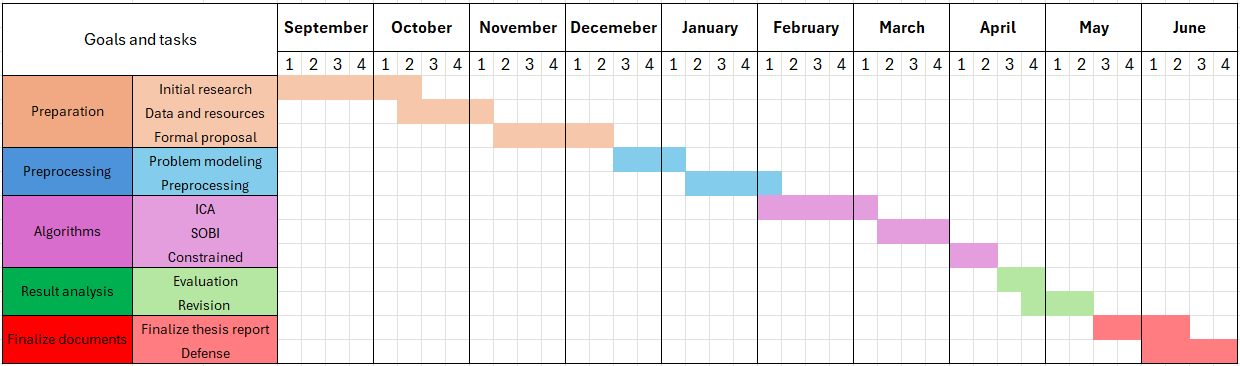
\includegraphics[width=\linewidth ]{figuras/chronogram_work.png}
    }
    \caption{Estimated work chronogram presented in the bachelor's thesis proposal.}
    \label{fig:chronogram}
\end{figure}

\section{Datasets}

The experiments performed in this thesis mainly use two distinct datasets: a real TMR EMG dataset and a synthetic dataset. The real dataset provides physiological EMG recordings, while the synthetic dataset enables controlled experiments that would be difficult to perform using publicly available data. Together, they allow the algorithms to be evaluated under realistic and simulated conditions.


\subsection{TMR patients dataset}
\label{subsec:tmr_dataset}
This dataset was collected as part of a study on myoelectric prosthesis hand grasp control in individuals with unilateral transradial amputation \cite{todd_kuiken_electromyography_2023}. This data is particularly relevant to this thesis since it provides physiological EMG data of patients \textbf{before and after reinnervation procedures} (TMR). This may be useful to both understand the characteristics of these signals as well as test the quality of separation algorithms on these signals. For clarity, the main characteristics of the dataset are summarized below. 
\begin{itemize}
    \item Six individuals with unilateral transradial amputation.
    \item EMG recorded before and after TMR surgery.
    \item 32 bipolar EMG channels placed along the residual forearm.
    \item Multiple hand, finger, wrist and rest movements.
    \item Each contraction was held for 2 seconds and repeated 8 times.
    \item Sampling frequency: \qty{1000}{Hz}.
\end{itemize}

To provide context for the possible relationships between EMG channels, Figure \ref{fig:TMR_tr2_diagram} illustrates the 32 channel electrode placement for patient TR2. For further reference, the electrode configurations of the remaining five patients are included in the original dataset description \cite{todd_kuiken_electromyography_2023}.

\begin{figure}[H]
    \centering
    \makebox[\textwidth][c]{%
        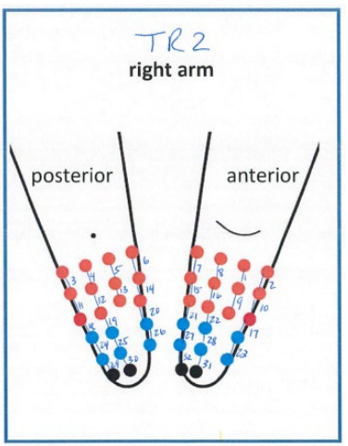
\includegraphics[width= 0.7\linewidth, height=7cm]{figuras/TMR_tr2_diagram.png}
    }
    \caption{Electrode placement for patient 2 of the TMR database. Both anterior and posterior views are shown for reference \cite{todd_kuiken_electromyography_2023}.}
    \label{fig:TMR_tr2_diagram}
\end{figure}
\subsection{Synthetic Dataset}
\label{subsec:synthetic_dataset}

This dataset is designed to test source separation under controlled conditions, especially when the muscle sources present clearly different activation patterns and signal amplitudes. Since EMG data with these specific characteristics are not easily available in public datasets, synthetic signals were generated following realistic EMG properties \cite{hamilton-wright_physiologically_2005}. This dataset is mainly used for the experiments presented in Chapter \ref{ch:sobi}. 

Figure \ref{fig:artificial_dataset_example} presents an example of the synthetic signals generated for the experimental tests.
Further details on the signal generation process are provided in \textbf{Appendix \ref{app:synthetic_signals}}.


\begin{figure}[H]
    \centering
    \makebox[\textwidth][c]{%
        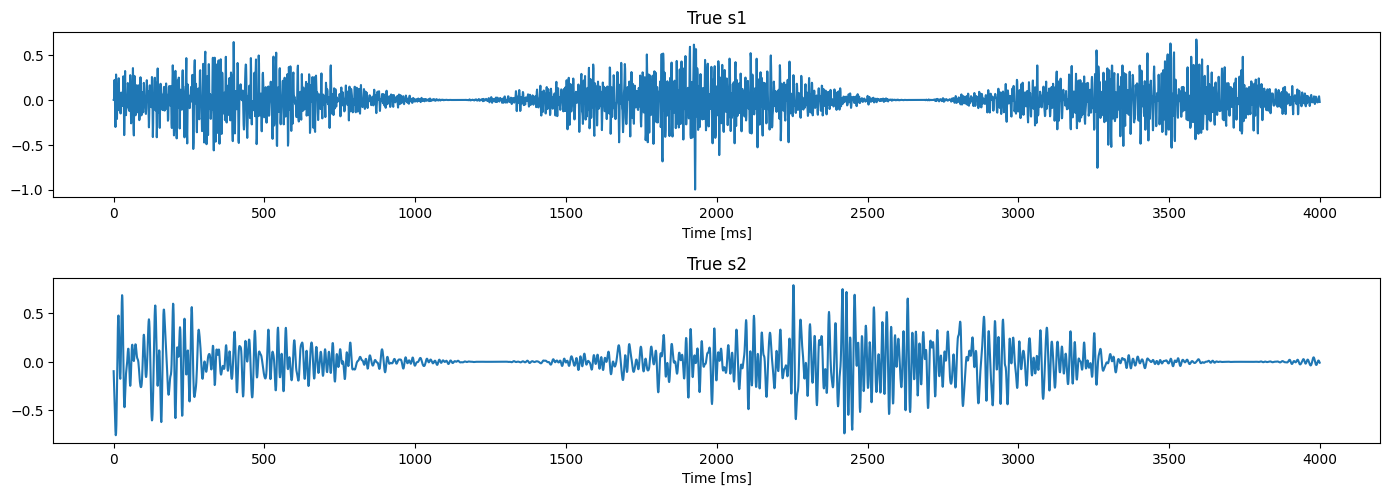
\includegraphics[width=\linewidth ]{figuras/artificial_dataset_example.png}
    }
    \caption{Example of synthetic signals generated for the artificial dataset.}
    \label{fig:artificial_dataset_example}
\end{figure}

\section{Experimental procedure}
This final subsection aims to establish and clarify the procedure followed when performing the experiments. An important clarification is that the experiments are performed with preprocessed signals, but the original sources are represented before the whitening step (see Chapter \ref{ch:preprocessing} for reference). It is also important to note that, since the synthetic dataset was designed for this thesis, it already includes the considerations mentioned in Subsection \ref{subsec:signal_selection} and \ref{subsec:signal_conditioning}. 



\subsection{Signal selection}
\label{subsec:signal_selection}
For simplification, the experiments performed throughout this thesis assume that the target flap related source is statistically independent from the donor muscle source. Therefore, when utilizing the TMR dataset, it is vital to perform the experiments with two independent EMG channels. Figure \ref{fig:channels_corr_matrix} illustrates the simplified correlation matrix for patient TR2 (post TMR surgery), which is the main subject selected for the experiments. 


\begin{figure}[H]
    \centering
    \makebox[\textwidth][c]{%
        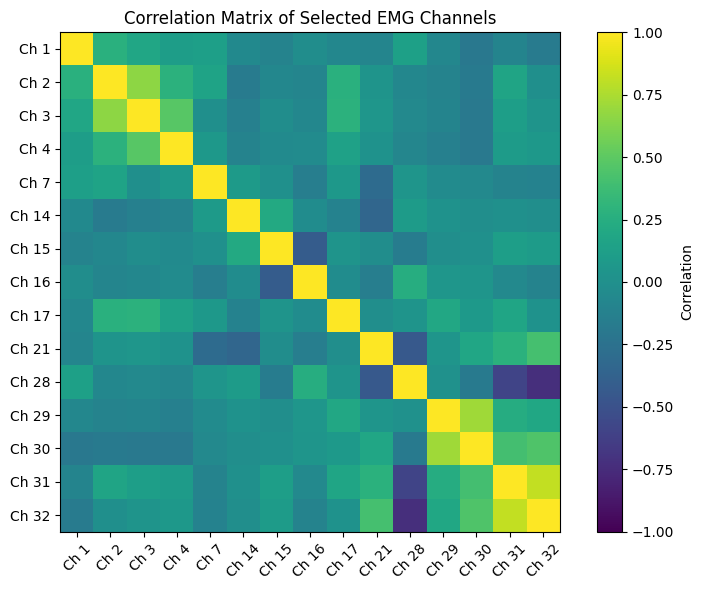
\includegraphics[width=\linewidth ]{figuras/channel_corr_matrix.png}
    }
    \caption{Correlation matrix of EMG channels in the TMR dataset. This figure is a reduced version of the original 32x32 correlation matrix.}
    \label{fig:channels_corr_matrix}
\end{figure}




Some adjacent channels show strong correlation, suggesting that they likely capture EMG activity from the same motor unit or nearby muscle regions. However, adjacency in channel number does not always lead to strong correlation, since the electrode configuration is not purely sequential as shown in Figure \ref{fig:TMR_tr2_diagram}. For example, channels 31 and 32 present one of the strongest correlations because they are physically close to each other. By contrast, the correlation between channels 16 and 17 is considerably less significant, despite being consecutive channel numbers.

For this reason, to satisfy the statistical independence condition, channels with neglectable correlations are selected for the experimentation. \textbf{Channels 4 and 21} are chosen for the main experiments shown in the algortihm chapters, while \textbf{channels 7 and 28} are used for the weak source and noise discussions.

\subsection{Signal conditioning}
\label{subsec:signal_conditioning}
Since the IIT study these EMG signals can be either activated simultaneously or at different times, it can be of interest to adapt the selected sources to reflect this key aspect. For this reason, arbitrary binary masks were applied to the TMR dataset signals to simulate this effect.
\textbf{See Appendix \ref{app:signal_coditioning} for reference.} Figure \ref{fig:signal_conditioning} shows a visual representation of how these EMG signals are adapted to satisfy this key aspect. 

\begin{figure}[H]
    \centering
    \makebox[\textwidth][c]{
        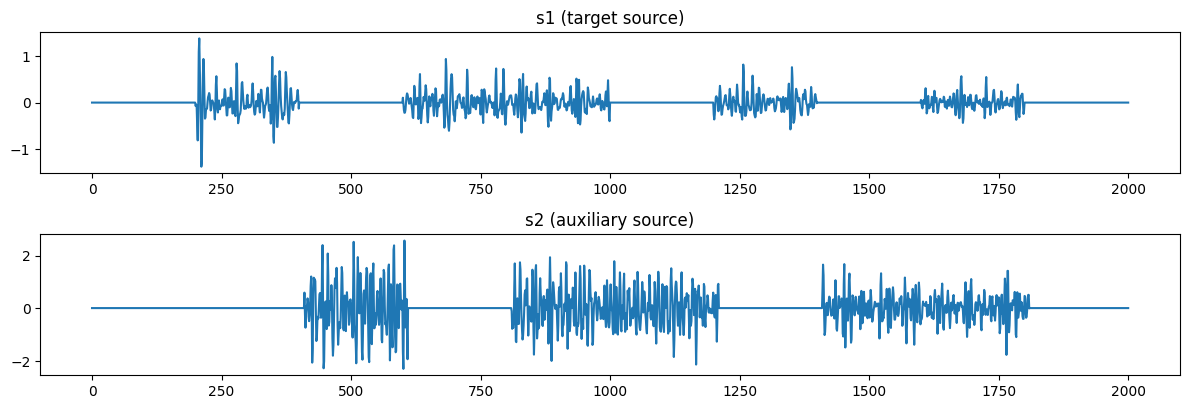
\includegraphics[width=\linewidth ]{figuras/signal_conditioning.png}
    }
    \caption{Example of the signal conditioning used to adapt the EMG signals from the TMR database to the considerations of this study. Signals are not always simultaneously activated. Instead their activations can be simultaneous or at the different periods.}
    \label{fig:signal_conditioning}
\end{figure}
\subsection{Mixing models}
To simulate the effect of muscles interference and reinnervation, different mixing models are considered in order to evaluate the separation performance under different scenarios.
Though chapter \ref{ch:problem_modeling} provides a more detailed discussion of the mixing models considered for this work, Figure \ref{fig:mixing_example} shows an example of how the signals selected in Figure \ref{fig:signal_conditioning} are combined following the model described in Section \ref{sec:weak_source_regime}, which is the model of main interest of this thesis. Equation \ref{eq:model_refresher} shows this model again for reference.

\begin{equation}
\left\{
\begin{aligned}
x_1(t) &= s_1(t) + \beta s_2(t-\tau) + n_1(t) \\
x_2(t) &= 0.01 s_1(t-\tau) + s_2(t) + n_2(t) 
\end{aligned}
\right.
\label{eq:model_refresher}
\end{equation}
\begin{figure}[H]
    \centering
    \makebox[\textwidth][c]{%
        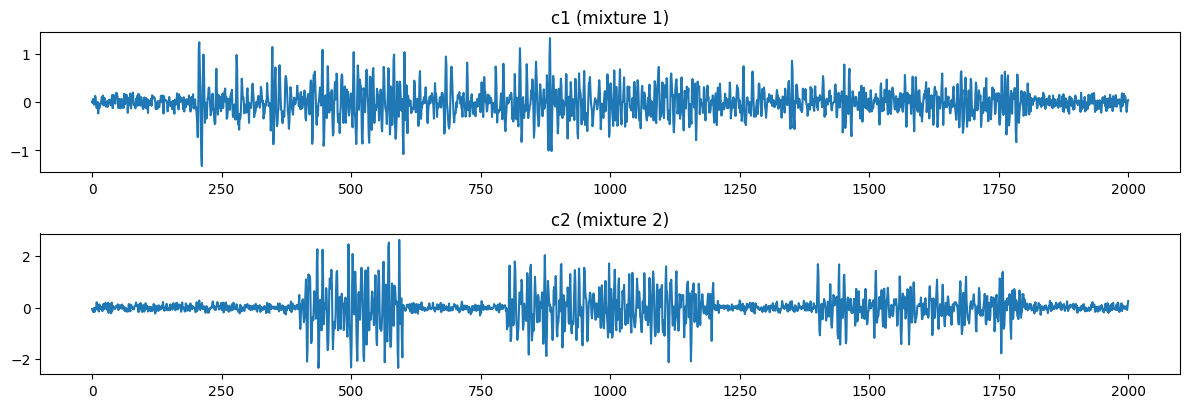
\includegraphics[width=\linewidth ]{figuras/mixing_example.png}
    }
    \caption{Example of source mixing following the model detailed in Section \ref{sec:weak_source_regime}. Parameters were set to $\beta=0.3$, $\sigma=0.1$ and $\tau=10$ms.}
    \label{fig:mixing_example}
\end{figure}

\subsection{Metrics}

Given the nature of this study, it is crucial to define a series of metrics to be able to quantify the performance of the mentioned algorithms in the different models and scenarios tested. Therefore, this subsection provides an enumeration of the metrics evaluated in this thesis, ranked by their importance when assessing the algorithms for the study. For clarification, the estimated source is $\hat{s}_1$ and the original source is $s_1$. 
The operator $\rho(\cdot,\cdot)$ denotes the Pearson correlation coefficient and $\mathrm{RMS}(\cdot)$ refers to the RMS envelope of a specific signal. Equation \ref{eq:metrics_formula} shows their mathematical expressions.
\begin{equation}
\begin{aligned}
\rho(x,y) &=
\frac{\operatorname{cov}(x,y)}
{\sigma_x \sigma_y}, \qquad
\mathrm{RMS}(x)[k] =
\sqrt{
\frac{1}{N_w}
\sum_{n=1}^{N_w} x_k^2[n]
}
\end{aligned}
\label{eq:metrics_formula}
\end{equation}

\begin{enumerate}
    \item \textbf{RMS envelope correlation}
    \[
    \operatorname{Corr}_{\mathrm{RMS}}(s_1,\hat{s}_1)
    =
    \rho\left(\mathrm{RMS}(s_1), \mathrm{RMS}(\hat{s}_1)\right)
    \]
This metric measures how well the estimated source preserves the activation pattern of the original signal through its RMS envelope rather than directly comparing the waveform sample by sample. Its scale varies from -1 to 1, where negative values indicate inverse relationship. 
\clearpage
    \item \textbf{Temporal correlation}
    \[
    \operatorname{Corr}(s_1,\hat{s}_1)
    =
    \rho(s_1,\hat{s}_1)
    \]
    This metric measures the similarity between the original and estimated raw waveforms. It evaluates how accurately the algorithm identifies the temporal structure of $s_1$ sample by sample. Its scale is the same as RMS envelope correlation.
    \item \textbf{Signal-to-noise ratio}
    \[
    \operatorname{SNR}_1 =\frac{\mathrm{Var}(s_1)}{\mathrm{Var}(error)}
    \]
    This metric measures the ratio of the power (or indirectly of variance) of the original target source and the power of the reconstruction error. Higher values indicate that the estimated source is closer to $s_1$ and contains less residual interference. 
\end{enumerate}

Out of the three presented metrics, the RMS envelope correlation is considered the most relevant metric because EMG-based prosthetic control mainly depends on the preservation of the activation pattern rather than on the exact reconstruction of each individual sample. However, if in some cases temporal correlation is optimized, this implies that activation patterns from the original sources are also recovered.
